\chapter{Fundamentação Teórica}
Este capítulo apresenta conceitos utilizados no desenvolvimento do trabalho, e portanto necessários para o correto entendimento do mesmo.

\section{Redes de Computadores}
A história dos computadores de grande escala começa em fevereiro de 1946 através da invenção do primeiro ``computador integrador numérico eletrônico'' \sigla{ENIAC}{\emph{Electronic Numerical Integrator and Computer}} \cite{Book_Jean2013}. Ele começou a ser desenvolvido anos antes, durante a Segunda Guerra Mundial, com a principal tarefa de auxiliar nos cálculos necessários para o fronte de batalha.

Em meados dos anos 50, com a popularização dos transistores, foi possível realizar uma imensa miniaturização dos circuitos eletrônicos possibilitando a criação de máquinas com altíssimo poder de processamento em um tamanho extremamente reduzido. Além disso, essas máquinas tornaram-se cada vez mais robustas e baratas, fazendo com que a posse e utilização de computadores pudesse ser disseminada alcançando os patamares atuais.

Neste sentido foi natural a necessidade da troca de informações/dados entre os diversos computadores existentes, o que claramente não representa maiores problemas caso os equipamentos em questão estejam fisicamente perto uns dos outros. Em contrapartida, é fácil imaginar a dificuldade de realização desta tarefa no caso em que estes equipamentos estivessem fisicamente distantes. Este é o cerne do problema que motivou a criação das redes de computadores.

Segundo \cite{Book_Kurose2013} uma rede de computadores nada mais é do que uma infraestrutura de comunicação que fornece serviços à aplicações distribuídas através de \emph{links} de comunicação contendo ``chaveadores de pacotes''. Sendo que uma rede pode ser essencialmente definida por seu tamanho, topologia e tecnologia de transmissão utilizada \cite{Book_Tanenbaum2003}. 
%Essas características, apesar de presentes em qualquer rede, são especialmente aplicáveis a redes locais (comumente chamadas de \sigla{LAN}{\emph{Local Area Network}}). 

\subsection{Tamanho}
Segundo \cite{Book_Tanenbaum2003} uma \sigla{LAN}{\emph{Local Area Network}} ou Rede Local possui tamanho restrito, e por isso seu desempenho é previsível. Ou seja, os piores tempos de transmissão de pacotes são conhecidos. 

Este tipo de rede pode possuir diversas topologias diferentes e pode ser encontrada nas mais diversas aplicações, desde residenciais, até industriais ou de automação. Uma das suas principais vantagens é a previsibilidade em termos de latência, visto que além de limitada e completamente conhecida ela normalmente não sofre alterações frequentes.

Uma Rede Metropolitana ou \sigla{MAN}{Metropolitan Area Network}, por sua vez, abrange uma cidade. Redes como esta foram inicialmente instaladas para sinais de TV a cabo. Atualmente elas são também utilizadas por provedores de internet \cite{Book_Tanenbaum2003}.

Uma Rede Geograficamente Distribuída ou \sigla{WAN}{Wide Area Network} abrange uma grande região como um país ou um continente e é responsável pelo roteamento dos pacotes entre as redes origem e destino. A forma e caminho utilizados para enviar as informações neste processo depende do algoritmo de roteamento utilizado. \cite{Book_Tanenbaum2003}

\subsection{Topologia}
Existem diversas formas de realizar a interconexão entre \emph{hosts} (dispositivos finais ou \emph{endpoints}). A topologia da rede depende de como esta interconexão é realizada. De maneira geral, podem-se destacar como mais comuns as topologias em barramento, anel, estrela, árvore e \emph{mesh}.

Uma topologia em barramento compartilha um mesmo meio para diversos \emph{hosts}. Todas as vezes que um deles deseja enviar alguma informação todos os equipamentos a recebem mas apenas o destinatário final à utiliza. Visto que o meio de comunicação é compartilhado é necessário existir alguma política de controle de acesso ao meio, prevenindo que mais de um \emph{endpoint} envie dados ao mesmo tempo, o que poderia gerar uma ``colisão'' embaralhando os dados de ambas as fontes. Este controle fica sob responsabilidade do protocolo de comunicação utilizado. A Figura \ref{fig_topologia_multiplo_barramento} representa uma rede conectada em barramento, percebe-se que o barramento central é compartilhado entre os diversos dispositivos conectados.

%\begin{figure}[!htb]
	%\centering
	%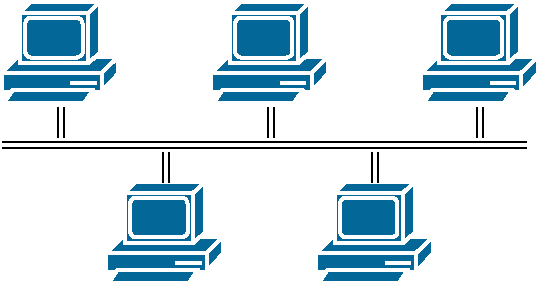
\includegraphics[width=0.2\textwidth]{./figuras/Topologia-Barramento.pdf} % <- formatos PNG, JPG e PDF
	%\caption[Exemplo de topologia em barramento]{Exemplo de topologia conectada em barramento. Percebe-se que o barramento central é compartilhado entre os diversos dispositivos conectados.}
	%\label{fig_topologia_barramento}
%\end{figure}

Na topologia em anel os \emph{hosts} são conectados através de um \emph{link} fechado, criando um anel. Cada estação é responsável por receber os dados em uma porta e encaminhá-los à outra até que esta alcance seu destino. Este tipo de rede fornece redundância já que as mensagens trocadas podem ser enviadas por mais de um caminho. A Figura \ref{fig_topologia_multiplo_barramento_anel} representa uma rede em anel, pode-se perceber que neste caso todos os equipamentos fazem parte da rede e precisam repetir os dados recebidos para os demais.

%\begin{figure}[!htb]
	%\centering
	%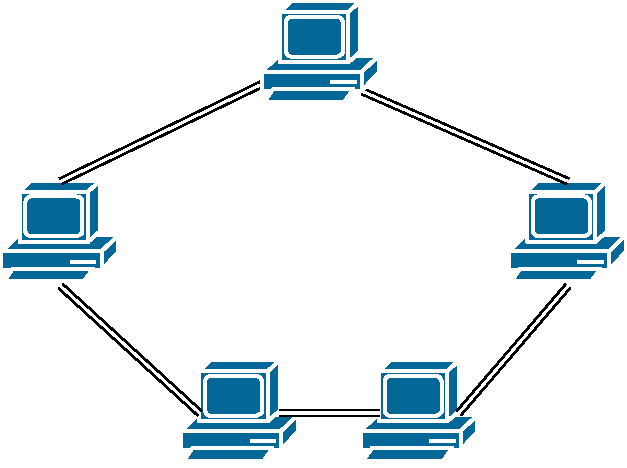
\includegraphics[width=0.2\textwidth]{./figuras/Topologia-Anel.pdf} % <- formatos PNG, JPG e PDF
	%\caption[Exemplo de topologia em anel]{Exemplo de topologia conectada em anel. Percebe-se que todos os equipamentos fazem parte da rede e precisam repetir os dados recebidos para os demais.}
	%\label{fig_topologia_anel}
%\end{figure}

A topologia estrela é muito utilizada em redes sem fio, visto que de maneira geral, todos os \emph{hosts} estão conectados a um ponto de acesso ou \sigla{AP}{Access Point}. Esse tipo de rede também pode ser facilmente encontrada em um meio cabeado, como no caso da utilização dos roteadores/switches residenciais, onde todos os \emph{hosts} são conectados a um mesmo equipamento responsável pela criação de uma LAN e interconexão com uma WAN. A Figura \ref{fig_topologia_multiplo_estrela} representa uma rede de topologia estrela, neste tipo de topologia todos os equipamentos estão ligados a um nó central, neste caso um \emph{switch}.

%\begin{figure}[!htb]
	%\centering
	%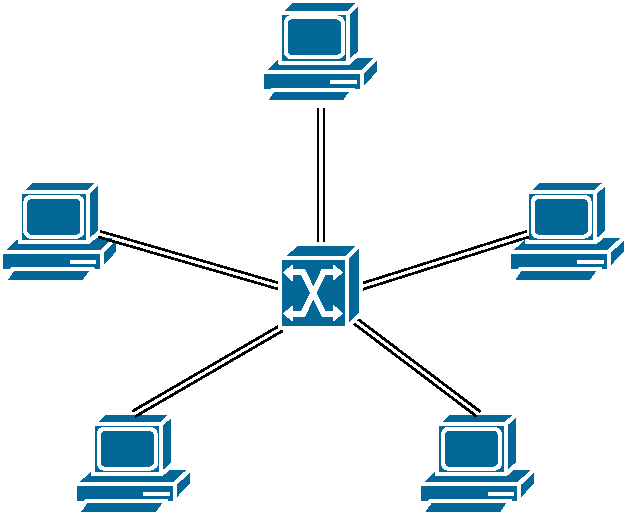
\includegraphics[width=0.2\textwidth]{./figuras/Topologia-Estrela.pdf} % <- formatos PNG, JPG e PDF
	%\caption[Exemplo de topologia em estrela]{Exemplo de topologia conectada em estrela. Percebe-se que todos os equipamentos estão ligados a um nó central, neste caso um \emph{switch}.}
	%\label{fig_topologia_estrela}
%\end{figure}

A topologia em árvore, talvez a mais recorrente em redes de computadores, é assim chamada pois pode ser reconhecida pelo seu aspecto onde o nó central representa a base da árvore e os diversos \emph{hosts} representam suas folhas. Basicamente trata-se de uma estrutura hierárquica de conexão entre várias redes e/ou sub-redes. A Figura \ref{fig_topologia_multiplo_arvore} ilustra esse tipo de topologia. Percebe-se que a topologia assemelha-se à interconexão de várias sub-redes através de equipamentos dedicados.

%\begin{figure}[!htb]
	%\centering
	%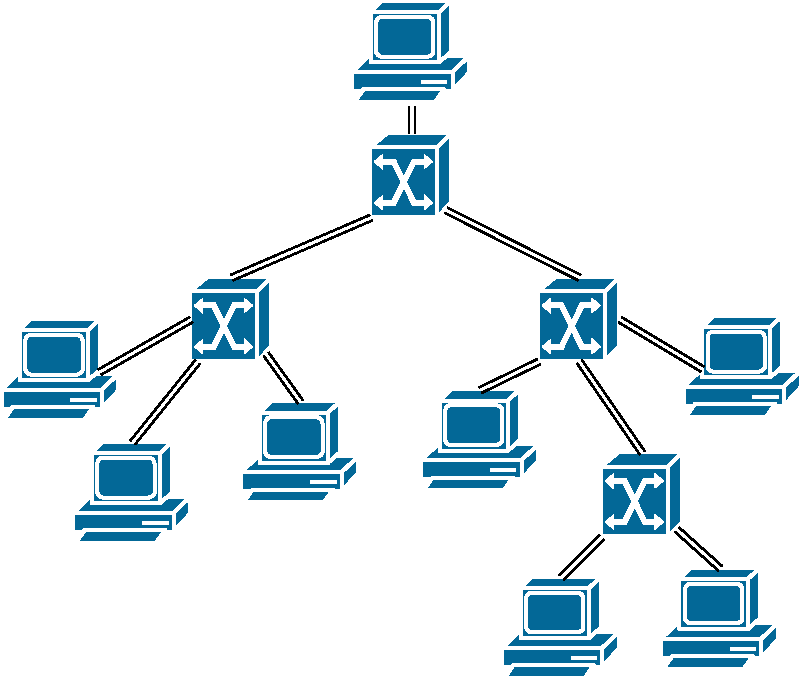
\includegraphics[width=0.2\textwidth]{./figuras/Topologia-Arvore.pdf} % <- formatos PNG, JPG e PDF
	%\caption[Exemplo de topologia em árvore]{Exemplo de topologia conectada em árvore. Percebe-se que a topologia assemelha-se à interconexão de várias sub-redes através de equipamentos dedicados.}
	%\label{fig_topologia_arvore}
%\end{figure}

A topologia em malha ou \emph{mesh} por sua vez, é caracterizada pela criação de uma rede grandemente (podendo chegar a ser plenamente) interconectada, formando diversos caminhos redundantes para a interligação entre a origem e o destino das mensagens. Fato que confere a este tipo de rede um elevado grau de disponibilidade, visto que mesmo em caso de falha de equipamentos ou da infraestrutura a comunicação não é necessariamente comprometida. A Figura \ref{fig_topologia_multiplo_mesh} ilustra uma rede \emph{mesh}. É possível notar que existem diversas rotas redundantes devido aos vários links estabelecidos entre os equipamentos da rede.

%\begin{figure}[!htb]
	%\centering
	%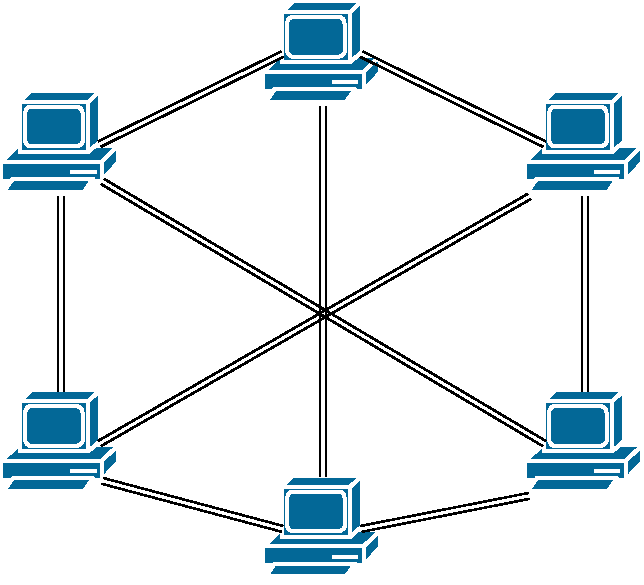
\includegraphics[width=0.2\textwidth]{./figuras/Topologia-Mesh.pdf} % <- formatos PNG, JPG e PDF
	%\caption[Exemplo de topologia em \emph{mesh}]{Exemplo de topologia conectada em \emph{mesh}. Percebe-se existem diversas rotas redundantes devido aos vários links estabelecidos entre os equipamentos da rede.}
	%\label{fig_topologia_mesh}
%\end{figure}

\begin{figure}[t!]
	\centering
	\begin{subfigure}[t]{0.4\textwidth}
		\centering
		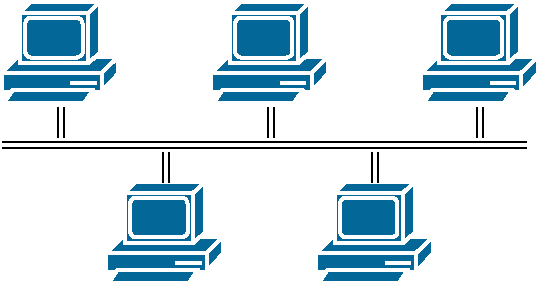
\includegraphics[width=4cm]{./figuras/Topologia-Barramento.pdf} % <- formatos PNG, JPG e PDF
		\caption{Topologia em barramento.}
		\label{fig_topologia_multiplo_barramento}
	\end{subfigure}%
	~
	\begin{subfigure}[t]{0.4\textwidth}
		\centering
		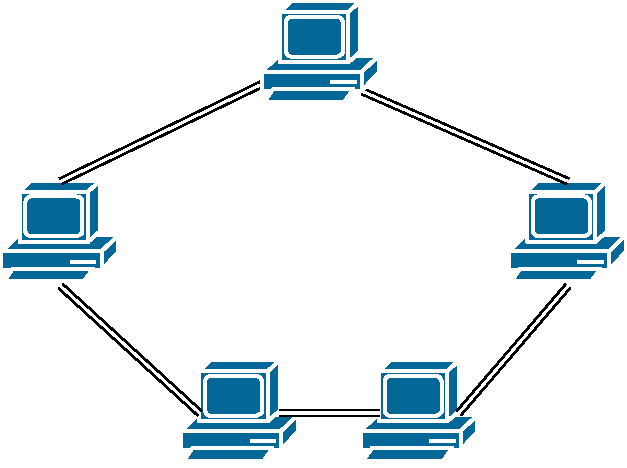
\includegraphics[width=4cm]{./figuras/Topologia-Anel.pdf} % <- formatos PNG, JPG e PDF
	\caption{Topologia em anel.}
	\label{fig_topologia_multiplo_barramento_anel}
	\end{subfigure}
	~
	\begin{subfigure}[t]{0.4\textwidth}
		\centering
		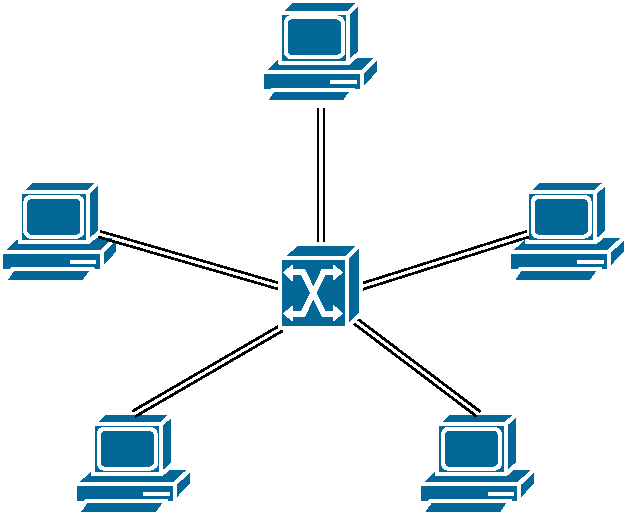
\includegraphics[width=4cm]{./figuras/Topologia-Estrela.pdf} % <- formatos PNG, JPG e PDF
	\caption{Topologia em estrela.}
	\label{fig_topologia_multiplo_estrela}
	\end{subfigure}
	~
	\begin{subfigure}[t]{0.4\textwidth}
		\centering
		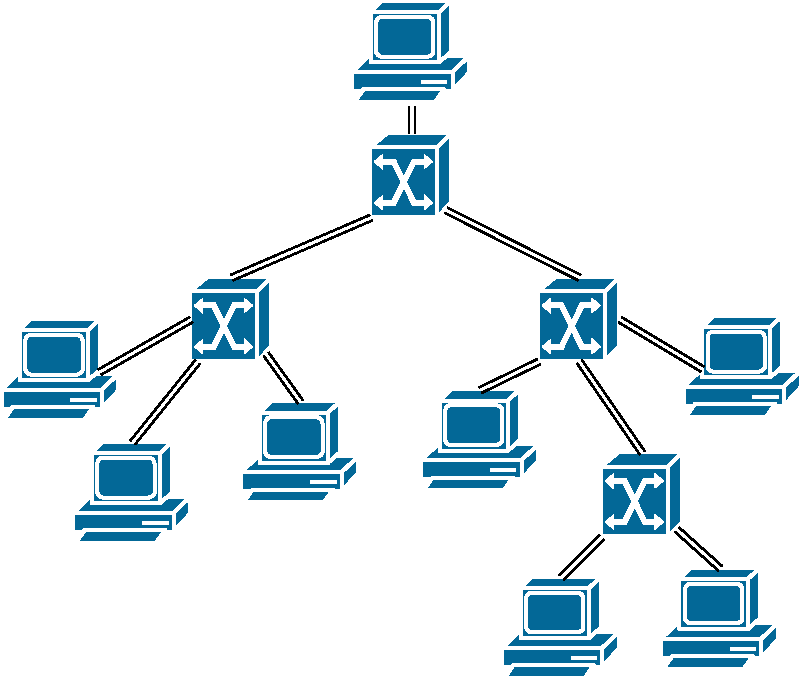
\includegraphics[width=4cm]{./figuras/Topologia-Arvore.pdf} % <- formatos PNG, JPG e PDF
	\caption{Topologia em árvore.}
	\label{fig_topologia_multiplo_arvore}
	\end{subfigure}
	~
	\begin{subfigure}[t]{0.4\textwidth}
		\centering
		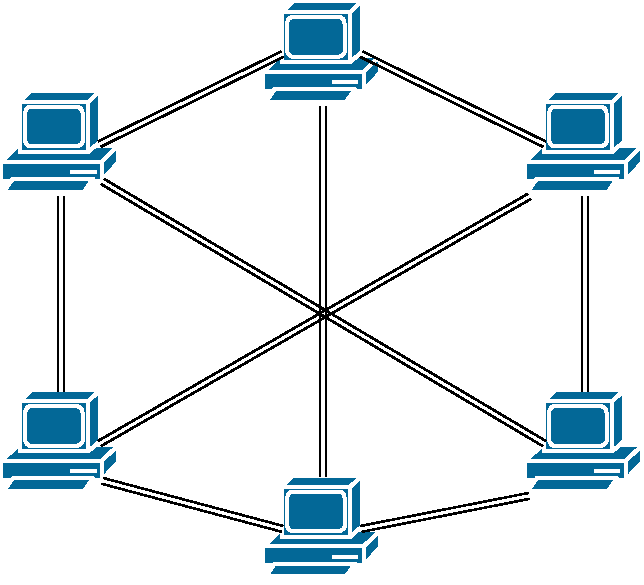
\includegraphics[width=4cm]{./figuras/Topologia-Mesh.pdf} % <- formatos PNG, JPG e PDF
	\caption{Topologia em \emph{mesh}.}
	\label{fig_topologia_multiplo_mesh}
	\end{subfigure}
	\caption{Tipos básicos de topologia}
	\label{fig_topologia_multiplo}
\end{figure}

\subsection{Tecnologia de Transmissão}
A tecnologia de transmissão está diretamente ligada ao meio físico utilizado, que não precisa ser necessariamente construído em cabos metálicos. Podem ser utilizados fibras ópticas, enlaces de micro-ondas, ondas infravermelhas, satélites de comunicação, entre outros \cite{Book_Tanenbaum2003}. 

Além disso, as redes de computadores podem, e comumente são, criadas através da interconexão de redes híbridas, ou seja, diferentes sub-redes criadas com tecnologias de transmissão distintas. Essas redes por sua vez têm diferentes taxas de transmissão e valores típicos de latência e demais parâmetros aos quais todos os pacotes que as atravessarem estarão submetidos \cite{Book_Kurose2013}. Logo, quando é necessário realizar uma comunicação entre \emph{hosts} em redes que utilizam tecnologias de transmissão diferentes é necessária a existência de algum tipo de mecanismo para regulação da velocidade de transferência de informação assim como políticas de garantia de entrega dos dados. Estes mecanismos são algumas das responsabilidades básicas dos protocolos de roteamento como o TCP/IP.